\documentclass[12pt,letterpaper]{article}

% Paquetes necesarios
\usepackage[utf8]{inputenc}
\usepackage[spanish,es-tabla]{babel}
\usepackage{geometry}
\usepackage{graphicx}
\usepackage{float}
\usepackage{setspace}
\usepackage{titlesec}
\usepackage{fancyhdr}
\usepackage{enumitem}
\usepackage{caption}
\usepackage{amsmath}
\usepackage{booktabs}
\usepackage{array}
\usepackage{xcolor}
\usepackage{tikz}
\usepackage{pgfplots}
\usepackage[hidelinks]{hyperref}

\usetikzlibrary{arrows.meta,positioning,shapes.geometric,calc}
\pgfplotsset{compat=1.18}

% Configuración de página
\geometry{
    top=2.5cm,
    bottom=2.5cm,
    left=3cm,
    right=2.5cm,
    headheight=14pt
}

% Configuración de encabezado y pie de página
\pagestyle{fancy}
\fancyhf{}
\fancyhead[L]{\small Control de Procesos Industriales}
\fancyhead[R]{\small Práctica \#4}
\fancyfoot[C]{\thepage}
\renewcommand{\headrulewidth}{0.4pt}
\renewcommand{\footrulewidth}{0.4pt}

% Configuración de espaciado
\setstretch{1.15}

\definecolor{uaqblue}{RGB}{26,64,112}
\definecolor{controlgreen}{RGB}{28,118,92}
\definecolor{softgray}{RGB}{245,247,250}

\begin{document}

% Portada
\begin{titlepage}
    \centering

    
\includegraphics[width=0.75\textwidth]{LOGOS.png}

    \vspace{2cm}

    {\LARGE\bfseries Universidad Autónoma de Querétaro\par}
    \vspace{0.5cm}
    {\Large Facultad de Ingeniería\par}
    \vspace{3cm}

    {\LARGE\bfseries Control de Procesos Industriales\par}
    \vspace{1cm}
    {\Large\textit{Práctica 04: Instrumentación: Controladores}\par}
    \vspace{1.5cm}

    {\large\bfseries Integrantes\par}
    \vspace{0.4cm}
    {\large
    \begin{tabular}{c}
        Luis Fernando Pérez Tellez \\
        Jesus Pablo Arteaga Silva \\
        Braulio Iván Gómez Ortiz \\
        Joselyn Gallegos Abreo \\
        Luis Alejandro Zeron Marin
    \end{tabular}
    \par}

    \vfill

    {\large Ing. Ramón Antonio González Hernández\par}
    \vspace{1cm}
    {\large Fecha: 25 de mayo de 2026\par}

\end{titlepage}

\pagestyle{fancy}

% ============================================================
% OBJETIVO
% ============================================================
\section*{Objetivo}

Que el alumno identifique, adquiera el conocimiento y habilidad en el manejo, configuración e instalación de los controladores dentro del campo de la instrumentación de los procesos industriales.

% ============================================================
% ACTIVIDADES
% ============================================================
\section*{Actividades}

\textbf{1.- Seminario de teoría y práctica donde se expliquen y comprendan los siguientes conceptos:}

\begin{itemize}[noitemsep]
    \item Definición de controlador.
    \item Características y tipos de controladores.
    \item Definición de los parámetros de configuración proporcional, derivativo e integral.
    \item Terminología y definiciones conceptuales aplicables a la instrumentación y al control de procesos.
\end{itemize}

% -----------------------------------------------------------
\subsection*{Controlador}

Un controlador es el elemento del lazo de control que compara la variable de proceso medida con el valor deseado o punto de ajuste, y calcula una acción correctiva para reducir el error. En instrumentación industrial, el controlador recibe la señal del transmisor, ejecuta una ley de control y entrega una señal de salida hacia el elemento final de control, normalmente una válvula, variador, resistencia, bomba o actuador \cite{smith2006}.

La variable controlada se identifica como PV (\textit{process variable}), el punto de ajuste como SP (\textit{set point}), la señal manipulada como MV (\textit{manipulated variable}) y el error como:

\begin{equation}
    e(t)=SP(t)-PV(t)
\end{equation}

% -----------------------------------------------------------
\subsection*{Características y Tipos de Controladores}

Los controladores se clasifican por su principio de operación, por la ley de control que ejecutan y por su integración dentro del sistema de instrumentación. En la industria de procesos se emplean controladores neumáticos, electrónicos, digitales, PLC, DCS y controladores embebidos en instrumentos Smart.

\begin{center}
\begin{tabular}{>{\bfseries}p{4.0cm} p{9.0cm}}
\toprule
\textbf{Tipo} & \textbf{Características principales} \\
\midrule
Neumático & Opera con señales de 3--15 psi. Es robusto y adecuado para áreas donde se desea evitar instrumentación eléctrica. \\
\addlinespace
Electrónico analógico & Opera con señales de 4--20 mA o 1--5 V. Permite mayor precisión y respuesta más rápida que el control neumático. \\
\addlinespace
Digital & Ejecuta algoritmos de control por software. Facilita alarmas, tendencias, comunicación, autodiagnóstico y ajuste remoto. \\
\addlinespace
PLC/DCS & Integra control de múltiples lazos, secuencias, interlocks, históricos y supervisión desde HMI o sala de control. \\
\bottomrule
\end{tabular}
\end{center}

Según la acción de control, los tipos más comunes son:

\begin{itemize}[itemsep=0.3em]
    \item \textbf{On-Off:} Actúa en dos estados. Es simple, pero genera oscilación alrededor del punto de ajuste.
    \item \textbf{Proporcional (P):} La salida cambia proporcionalmente al error. Mejora la respuesta, aunque puede dejar error permanente.
    \item \textbf{Proporcional-Integral (PI):} Elimina el error permanente mediante acción integral. Es el más usado en lazos de presión, flujo, nivel y temperatura.
    \item \textbf{Proporcional-Integral-Derivativo (PID):} Agrega anticipación por derivada. Se usa cuando se requiere mejorar la respuesta transitoria y el proceso permite medir sin ruido excesivo.
\end{itemize}

% -----------------------------------------------------------
\subsection*{Parámetros de Configuración de Controladores}

La forma paralela ideal del controlador PID se expresa como \cite{ogata2010}:

\begin{equation}
    m(t)=K_c\left[e(t)+\frac{1}{T_i}\int_0^t e(\tau)d\tau + T_d\frac{de(t)}{dt}\right] + m_0
\end{equation}

donde $m(t)$ es la salida del controlador, $K_c$ es la ganancia proporcional, $T_i$ es el tiempo integral, $T_d$ es el tiempo derivativo y $m_0$ es la salida de sesgo.

\begin{center}
\begin{tabular}{>{\bfseries}p{3.8cm} p{9.2cm}}
\toprule
\textbf{Parámetro} & \textbf{Efecto en el lazo de control} \\
\midrule
Ganancia proporcional $K_c$ & Aumenta la fuerza de corrección ante un error. Si es demasiado baja, el sistema responde lento; si es demasiado alta, puede oscilar. \\
\addlinespace
Tiempo integral $T_i$ & Corrige el error acumulado y elimina el offset. Un $T_i$ muy pequeño puede producir sobreimpulso y oscilación. \\
\addlinespace
Tiempo derivativo $T_d$ & Anticipa cambios rápidos del error. Ayuda en algunos procesos lentos, pero amplifica ruido de medición. \\
\addlinespace
Banda proporcional PB & Forma alternativa de expresar la ganancia: $PB=100/K_c$ cuando $K_c$ se expresa en unidades normalizadas. \\
\bottomrule
\end{tabular}
\end{center}

% -----------------------------------------------------------
\subsection*{Terminología Aplicable a Control de Procesos}

\begin{itemize}[itemsep=0.25em]
    \item \textbf{PV:} Variable medida del proceso.
    \item \textbf{SP:} Valor deseado de operación.
    \item \textbf{MV:} Variable manipulada por el controlador.
    \item \textbf{Offset:} Error permanente entre PV y SP.
    \item \textbf{Perturbación:} Cambio externo que afecta el proceso, por ejemplo una variación de demanda.
    \item \textbf{Tiempo muerto:} Retardo entre una acción de control y su efecto visible en la variable medida.
    \item \textbf{Constante de tiempo:} Tiempo característico de respuesta del proceso ante un cambio.
    \item \textbf{Sobreimpulso:} Exceso temporal de la PV por encima del SP después de una corrección.
    \item \textbf{Estabilidad:} Capacidad del sistema para regresar a una condición controlada sin oscilación creciente.
\end{itemize}

\newpage

% ============================================================
% CASO 1
% ============================================================
\section*{Caso 1: Sistema Teórico de Control de Presión}

\subsection*{Descripción del Proceso}

Se propone un sistema de control de presión para un tanque pulmón de nitrógeno destinado al suministro de soplado en una tubería de transporte de pellets de polímero hacia silos de almacenamiento. El tanque pulmón funciona como volumen amortiguador: almacena gas comprimido, reduce fluctuaciones de presión y permite que el controlador mantenga el suministro dentro de un margen seguro.

\begin{figure}[H]
\centering
\begin{tikzpicture}[
    node distance=1.6cm,
    block/.style={draw, rounded corners, align=center, minimum height=1.0cm, minimum width=2.6cm, fill=softgray},
    inst/.style={draw, circle, align=center, minimum size=1.1cm, fill=white},
    valve/.style={draw, regular polygon, regular polygon sides=3, shape border rotate=90, minimum size=0.9cm, fill=white},
    line/.style={-Latex, thick}
]
    \node[block] (supply) {Suministro\\N$_2$\\80,000 SCFH};
    \node[valve, right=1.5cm of supply] (pcv) {};
    \node[above=0.15cm of pcv] {\small PCV};
    \node[block, right=1.6cm of pcv, minimum width=2.9cm] (tank) {Tanque pulmón\\SP = 115 psig};
    \node[block, right=1.6cm of tank] (load) {Transporte\\de pellets\\40,000 SCFH};
    \node[inst, above=1.7cm of tank] (pt) {PT};
    \node[inst, above=1.7cm of pcv] (pic) {PIC};

    \draw[line] (supply) -- (pcv);
    \draw[line] (pcv) -- (tank);
    \draw[line] (tank) -- (load);
    \draw[line] (tank) -- (pt);
    \draw[line] (pt) -- node[above]{\small 4--20 mA} (pic);
    \draw[line] (pic) -- node[right]{\small 4--20 mA} (pcv);
\end{tikzpicture}
\caption{Configuración propuesta del lazo de control de presión en tanque pulmón de nitrógeno}
\label{fig:lazo_presion}
\end{figure}

% -----------------------------------------------------------
\subsection*{Datos del Problema}

\begin{center}
\begin{tabular}{>{\bfseries}p{5cm} p{7cm}}
\toprule
\textbf{Variable} & \textbf{Valor} \\
\midrule
Fluido & Nitrógeno \\
Temperatura & 65 $^\circ$F \\
Presión de operación & 115 psig \\
Flujo requerido & 40,000 SCFH \\
Tiempo de arranque & 10 min \\
Límite mínimo antes de paro & $-3\%$ de la presión de operación \\
Capacidad del suministro & 80,000 SCFH a 115 psig \\
Tubería & 3 pulgadas, cédula 40, longitud 80 m \\
\bottomrule
\end{tabular}
\end{center}

La presión mínima permisible antes del paro del sistema es:

\begin{equation}
    P_{min}=115(1-0.03)=111.55\ \text{psig}
\end{equation}

El margen disponible de presión es:

\begin{equation}
    \Delta P=115-111.55=3.45\ \text{psi}
\end{equation}

En presión absoluta:

\begin{equation}
    P_1=115+14.7=129.7\ \text{psia}
\end{equation}

\begin{equation}
    P_2=111.55+14.7=126.25\ \text{psia}
\end{equation}

% -----------------------------------------------------------
\subsection*{Selección del Controlador}

Para un tanque pulmón de gas se recomienda utilizar un controlador PI de presión. La acción proporcional corrige cambios inmediatos de presión y la acción integral elimina el error permanente. La acción derivativa no se considera necesaria como ajuste inicial porque la medición de presión puede contener ruido y porque el volumen del tanque ya aporta amortiguamiento al proceso.

La configuración propuesta es:

\begin{center}
\begin{tabular}{>{\bfseries}p{4.4cm} p{8.4cm}}
\toprule
\textbf{Elemento} & \textbf{Configuración recomendada} \\
\midrule
Controlador & PI digital o controlador de presión en PLC/DCS \\
Variable controlada & Presión del tanque pulmón \\
Punto de ajuste & 115 psig \\
Acción de control & Inversa para válvula de entrada aire-abre: si baja la presión, aumenta la salida del controlador \\
Salida del controlador & 4--20 mA hacia posicionador o convertidor I/P de la válvula PCV \\
Alarma baja & 111.55 psig \\
Paro por baja presión & Igual o menor a 111.55 psig, con retardo de seguridad definido por operación \\
Ganancia inicial $K_c$ & 2.0 \\
Tiempo integral $T_i$ & 60 s \\
Tiempo derivativo $T_d$ & 0 s \\
\bottomrule
\end{tabular}
\end{center}

Estos parámetros se consideran valores iniciales de arranque. El ajuste final debe obtenerse mediante prueba de escalón en el skid o por identificación del proceso, verificando estabilidad, bajo sobreimpulso y recuperación rápida ante cambios de demanda.

% -----------------------------------------------------------
\subsection*{Dimensionamiento del Tanque Pulmón}

Se dimensiona el volumen conservador requerido suponiendo que durante el arranque el tanque debe sostener el flujo de demanda durante 10 minutos sin que la presión caiga más de 3\%. El volumen estándar requerido es:

\begin{equation}
    V_{std}=Q\,t=(40{,}000\ \text{SCFH})\left(\frac{10}{60}\ \text{h}\right)=6{,}666.7\ \text{SCF}
\end{equation}

Para un gas ideal en un tanque de volumen fijo:

\begin{equation}
    V_{std}=V_{tanque}\left(\frac{P_1-P_2}{P_{std}}\right)\left(\frac{T_{std}}{T_{tanque}}\right)
\end{equation}

Despejando el volumen físico del tanque:

\begin{equation}
    V_{tanque}=V_{std}\left(\frac{P_{std}}{P_1-P_2}\right)\left(\frac{T_{tanque}}{T_{std}}\right)
\end{equation}

Con $P_{std}=14.7$ psia, $T_{std}=60+459.67=519.67\,^\circ R$ y $T_{tanque}=65+459.67=524.67\,^\circ R$:

\begin{equation}
    V_{tanque}=6{,}666.7\left(\frac{14.7}{3.45}\right)\left(\frac{524.67}{519.67}\right)
\end{equation}

\begin{equation}
    V_{tanque}=28{,}700\ \text{ft}^3
\end{equation}

Conversión a metros cúbicos:

\begin{equation}
    V_{tanque}=28{,}700(0.0283168)=812.8\ \text{m}^3
\end{equation}

La tubería de 3 pulgadas cédula 40 tiene diámetro interno aproximado de 3.068 pulgadas. Su volumen físico es:

\begin{equation}
    V_{tuberia}=\frac{\pi D_i^2}{4}L
\end{equation}

\begin{equation}
    V_{tuberia}=\frac{\pi(0.2557\ \text{ft})^2}{4}(262.47\ \text{ft})=13.47\ \text{ft}^3
\end{equation}

El gas utilizable de la línea dentro del margen de 3.45 psi es aproximadamente:

\begin{equation}
    V_{std,linea}=13.47\left(\frac{3.45}{14.7}\right)\left(\frac{519.67}{524.67}\right)=3.13\ \text{SCF}
\end{equation}

La contribución de la tubería es despreciable frente a los 6,666.7 SCF requeridos durante el arranque. Por lo tanto, si se exige autonomía completa del tanque durante 10 minutos con solo 3\% de caída de presión, el volumen necesario resulta muy grande y poco práctico.

\subsection*{Interpretación de Ingeniería}

El suministro disponible tiene capacidad de 80,000 SCFH, mientras que el consumo del proceso es de 40,000 SCFH. Esto significa que, con el suministro activo, existe una reserva de capacidad del 100\% respecto a la demanda. Por ello, la función principal del tanque no debe ser sostener por sí solo los 10 minutos de consumo, sino amortiguar variaciones rápidas mientras la válvula de control y el suministro corrigen la presión.

Para asegurar que el sistema no pare por baja presión se recomienda:

\begin{itemize}[itemsep=0.25em]
    \item Mantener la válvula PCV dimensionada para al menos 80,000 SCFH a las condiciones de operación.
    \item Operar normalmente alrededor de 50\% de apertura para conservar margen de corrección.
    \item Configurar alarma baja antes del paro, por ejemplo a 113 psig, y paro a 111.55 psig.
    \item Ejecutar arranque gradual del transporte de pellets para evitar demanda instantánea máxima.
    \item Ajustar el controlador PI con prueba de escalón para evitar oscilación y caída excesiva de presión.
\end{itemize}

\newpage

% ============================================================
% CASO 2
% ============================================================
\section*{Caso 2: Práctica Física en el Sistema de Tanques}

\subsection*{Descripción del Sistema}

En la práctica se desarrolló el control de un sistema de aire. El arreglo consistía en una entrada de aire condicionada por un rotámetro, una válvula de control encargada de regular la entrada de aire, un tanque pulmón conectado a un tanque principal y una salida también condicionada por otro rotámetro.

El objetivo de control fue manipular el paso de aire por la válvula para que la presión del tanque pulmón alcanzara y mantuviera una presión previamente definida. Para ello se utilizó el DCS DeltaV, el cual recibe la señal analógica de un transmisor de presión conectado al tanque pulmón. Esta medición entra a un bloque PID; el controlador calcula una salida de control y la envía hacia un transductor I/P, que convierte la señal eléctrica en señal neumática para accionar la válvula de entrada de aire.

\begin{figure}[H]
\centering
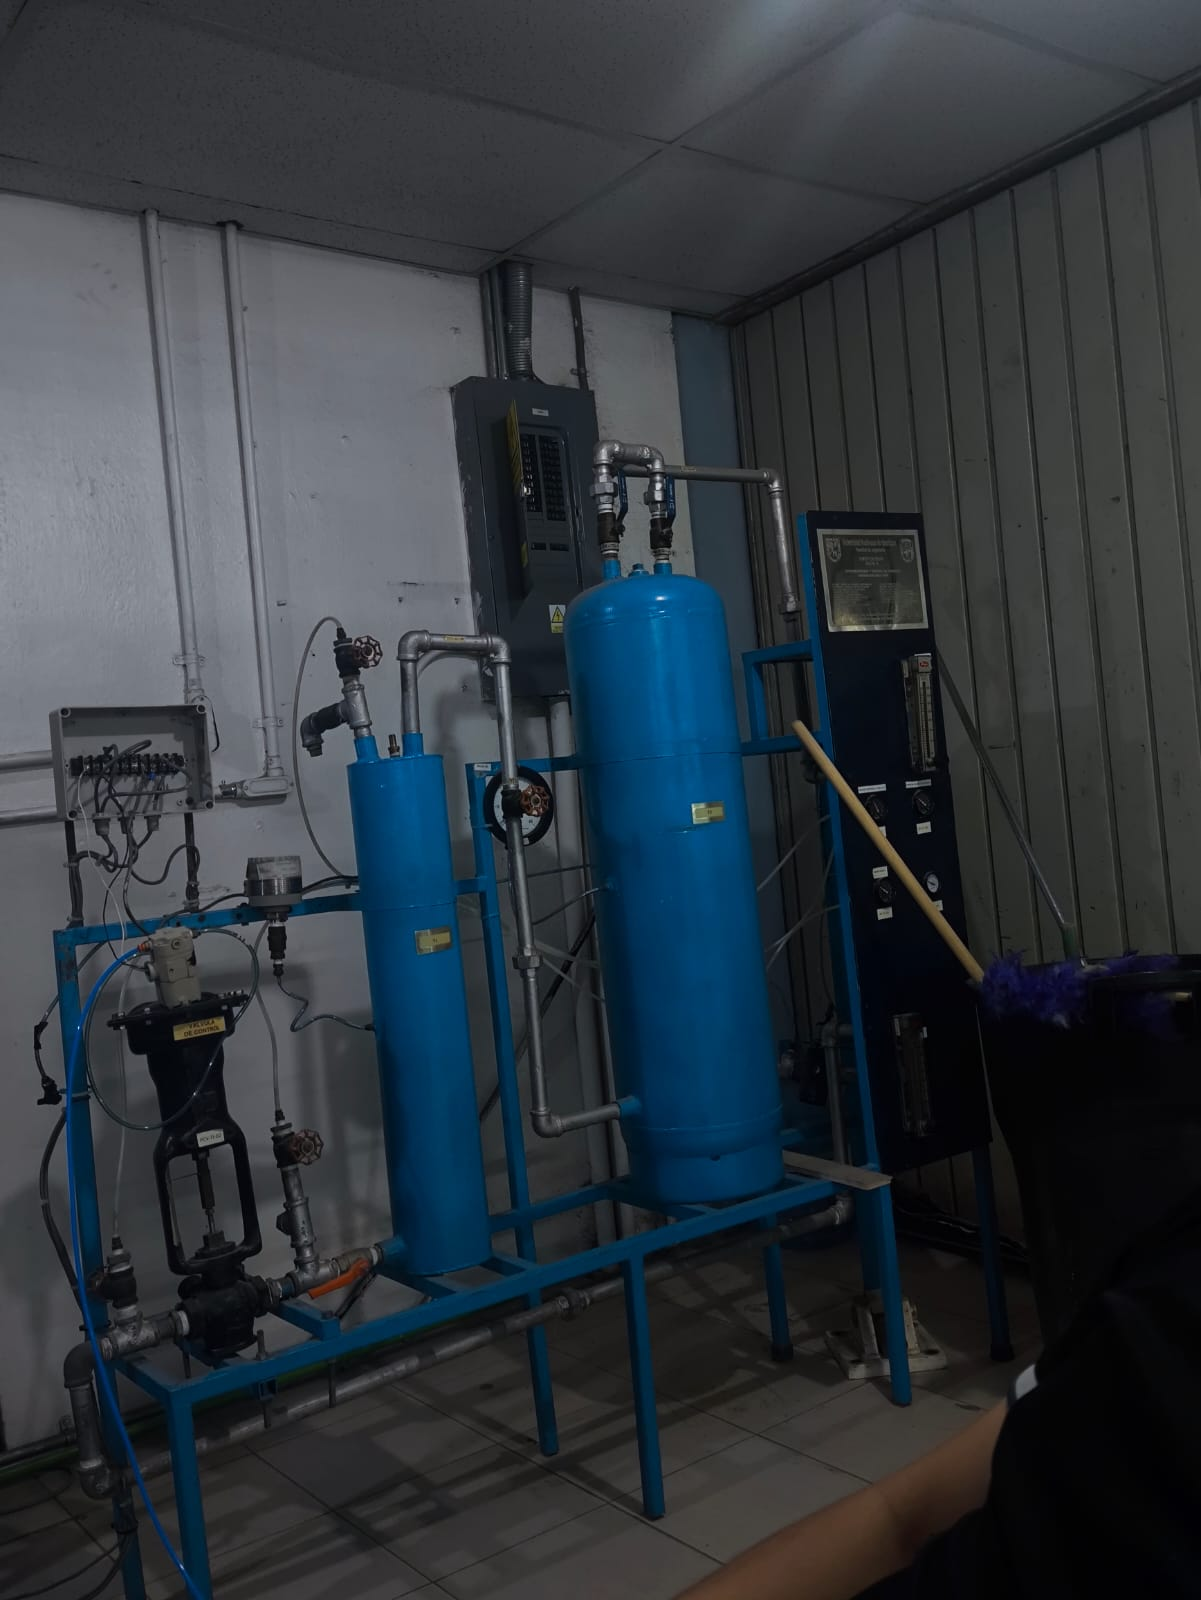
\includegraphics[width=0.64\textwidth]{figuras/skid_tanques.jpeg}
\caption{Sistema físico de tanques, rotámetros, válvula de control e instrumentación neumática}
\label{fig:skid_fisico}
\end{figure}

En la Figura \ref{fig:skid_fisico} se observa el skid utilizado en laboratorio. A la izquierda se identifica la zona de instrumentación y la válvula de control; al centro se encuentran el tanque pulmón y el tanque principal; y a la derecha se ubica el panel de operación con rotámetros y manómetros. El sistema permite modificar tanto la entrada como la salida de aire, por lo que es posible provocar cambios en la dinámica del proceso y observar la respuesta del controlador.

\begin{figure}[H]
\centering
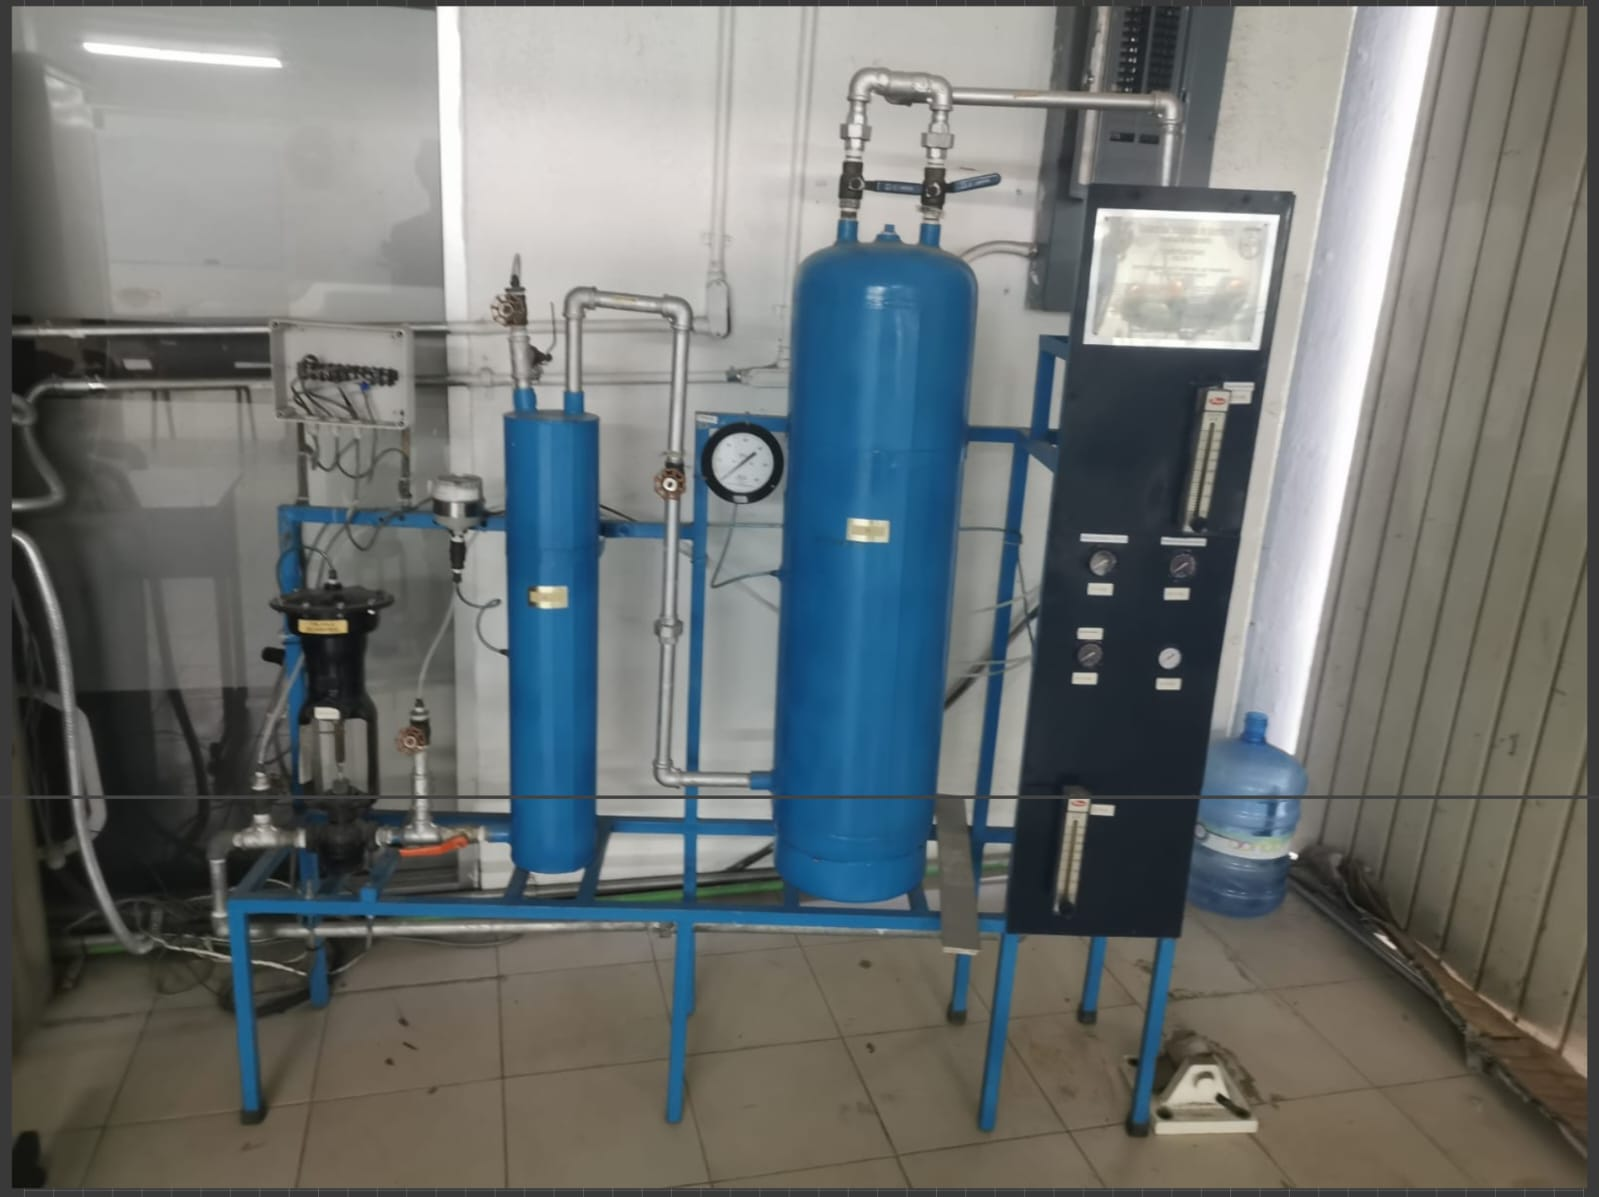
\includegraphics[width=0.88\textwidth]{figuras/tanques_general.jpeg}
\caption{Vista frontal del sistema: válvula de control, tanque pulmón, tanque principal, rotámetros y panel de operación}
\label{fig:tanques_general}
\end{figure}

La Figura \ref{fig:tanques_general} permite identificar con mayor claridad la distribución física del sistema. En la parte izquierda se aprecia la válvula de control neumática y su instrumentación asociada; al centro se observa el tanque pulmón de menor volumen y, a su derecha, el tanque principal. En el panel negro se ubican los rotámetros y manómetros utilizados para establecer condiciones de entrada y salida de aire durante la sintonización.

% -----------------------------------------------------------
\subsection*{DTI del Sistema de Tanques}

El DTI elaborado durante la práctica se replicó en TikZ para representar de forma ordenada el flujo de aire, los tanques, la instrumentación y las señales de control. El croquis original se conserva como referencia en la Figura \ref{fig:dti_referencia}.

\begin{figure}[H]
\centering
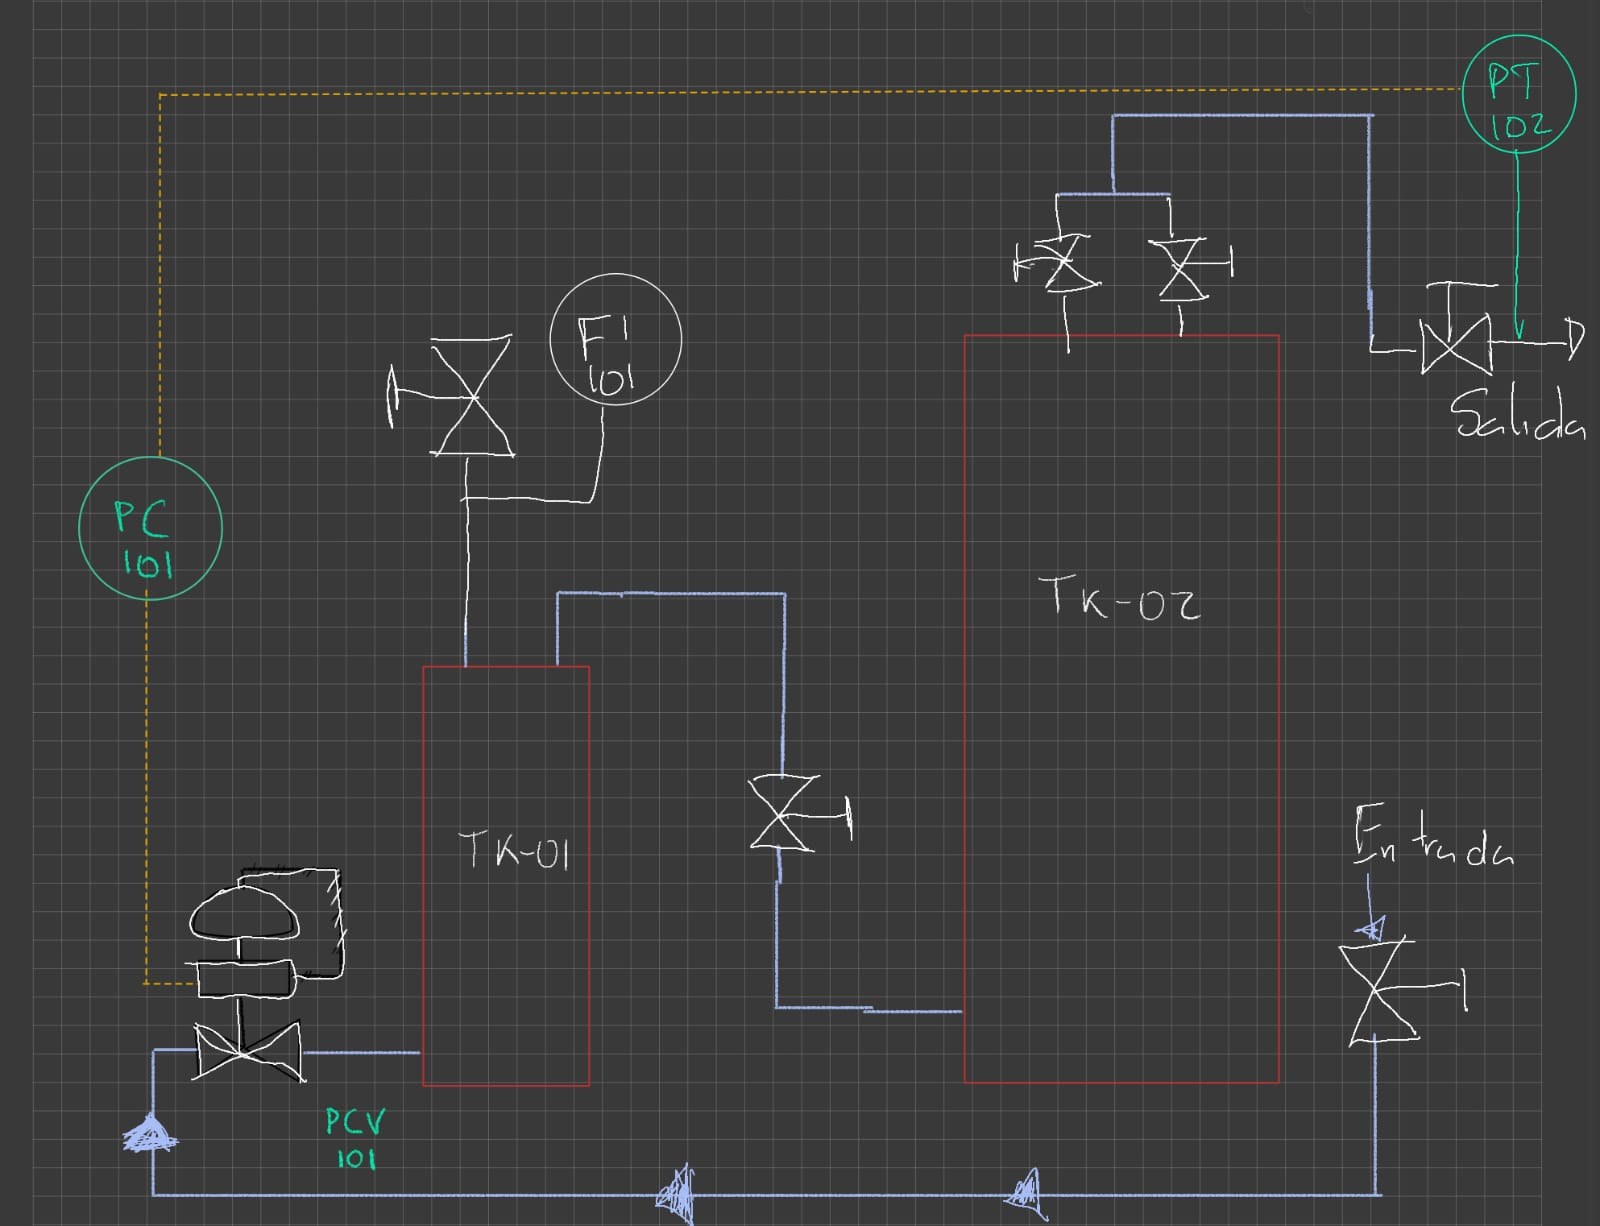
\includegraphics[width=0.92\textwidth]{figuras/dti_referencia.jpeg}
\caption{Croquis de referencia del DTI elaborado durante la práctica}
\label{fig:dti_referencia}
\end{figure}

\begin{figure}[H]
\centering
\resizebox{0.98\textwidth}{!}{%
\begin{tikzpicture}[
    pipe/.style={draw=blue!65, very thick},
    signal/.style={draw=controlgreen, very thick, -Latex},
    ctrl/.style={draw=yellow!70!black, very thick, dashed},
    vessel/.style={draw=red!70!black, very thick, minimum width=1.6cm, minimum height=4.4cm, align=center},
    tankbig/.style={draw=red!70!black, very thick, minimum width=2.3cm, minimum height=5.6cm, align=center},
    inst/.style={draw=controlgreen, very thick, circle, minimum size=1.35cm, align=center, fill=white},
    lab/.style={font=\small},
    valve/.style={draw=black, very thick, bowtie, minimum width=0.9cm, minimum height=0.55cm, fill=white}
]
    \tikzset{
        bowtie/.style={
            path picture={
                \draw[very thick] (path picture bounding box.south west) -- (path picture bounding box.center) -- (path picture bounding box.north west);
                \draw[very thick] (path picture bounding box.south east) -- (path picture bounding box.center) -- (path picture bounding box.north east);
            }
        }
    }

    % Equipos principales
    \node[vessel] (tk01) at (0,0) {TK-01};
    \node[tankbig] (tk02) at (5.6,0.2) {TK-02};

    % Línea principal de entrada y salida
    \draw[pipe,-Latex] (-4.7,-3.1) -- (-3.1,-3.1) node[midway, below=0.18cm, lab]{Entrada de aire};
    \node[valve] (pcv) at (-2.45,-3.1) {};
    \node[below=0.58cm of pcv, lab, text=controlgreen] {PCV-101};
    \draw[pipe] (-2.0,-3.1) -- (tk01.south west);
    \draw[pipe] (tk01.north) -- ++(0,1.1) -| (-2.45,-1.0);
    \node[valve] (vin) at (-2.45,-1.0) {};
    \node[inst] (fi) at (-0.1,3.4) {FI\\101};
    \draw[pipe] (-2.45,-0.72) |- (fi.west);

    % Interconexión entre tanques
    \draw[pipe] (tk01.north east) -- ++(0.9,0) |- (2.7,-0.15);
    \node[valve] (vinter) at (2.7,-0.15) {};
    \draw[pipe] (2.7,-0.45) |- (tk02.west);

    % Venteos/manifold superior de TK-02
    \draw[pipe] (tk02.north west) -- ++(0,1.1) -- ++(1.4,0);
    \node[valve] (vtop1) at (4.95,3.2) {};
    \node[valve] (vtop2) at (6.25,3.2) {};
    \draw[pipe] (vtop1) -- ++(0,-0.75);
    \draw[pipe] (vtop2) -- ++(0,-0.75);
    \draw[pipe] (6.25,3.2) -- ++(1.65,0) |- (8.6,1.9);

    % Salida
    \node[valve] (vout) at (8.6,1.9) {};
    \draw[pipe,-Latex] (vout) -- ++(1.25,0) node[right, lab]{Salida};
    \node[inst] (pst) at (9.1,4.1) {PST\\102};
    \draw[signal] (pst.south) -- (vout.north);

    % Controlador y señal
    \node[inst] (pc) at (-4.6,1.6) {PC\\101};
    \draw[ctrl] (pc.south) |- (pcv.west);
    \draw[ctrl] (pc.north) -- ++(0,2.3) -- ++(12.2,0) -- (pst.west);

    % Etiquetas de línea
    \node[lab, align=center] at (3.25,-1.15) {Válvula de\\interconexión};
    \node[lab, above] at (5.6,3.55) {Válvulas superiores};
\end{tikzpicture}
}
\caption{DTI replicado del sistema de control de presión en tanques}
\label{fig:dti_tikz}
\end{figure}

En la Figura \ref{fig:dti_tikz}, las líneas azules representan el recorrido físico del aire, las líneas verdes representan señales de medición o instrumentación asociada y la línea amarilla punteada representa la señal de control. El controlador PC-101 recibe la información de presión del sistema y actúa sobre la válvula PCV-101 para regular la entrada de aire al tanque pulmón.

\begin{center}
\small
\begin{tabular}{>{\bfseries}p{2.8cm} p{10cm}}
\toprule
\textbf{Elemento} & \textbf{Descripción funcional} \\
\midrule
PCV-101 & Válvula de control de entrada. Modula el paso de aire hacia el sistema de tanques de acuerdo con la salida del controlador. \\
\addlinespace
PC-101 & Controlador de presión implementado en DeltaV. Compara SP contra PV y genera la CV que gobierna la válvula de control. \\
\addlinespace
FI-101 & Indicador de flujo asociado a la entrada del sistema. Permite verificar la condición de alimentación de aire durante la práctica. \\
\addlinespace
TK-01 & Tanque pulmón. Es el recipiente donde se busca regular la presión y amortiguar cambios rápidos de flujo. \\
\addlinespace
TK-02 & Tanque principal conectado al tanque pulmón. Aumenta el volumen del sistema y modifica su respuesta dinámica. \\
\addlinespace
PST-102 & Transmisor/interruptor de presión de salida. Proporciona referencia de presión para supervisión y protección del sistema. \\
\addlinespace
Rotámetros & Instrumentos de entrada y salida utilizados para ajustar manualmente los flujos y generar perturbaciones controladas. \\
\bottomrule
\end{tabular}
\end{center}

El transmisor entrega la variable de proceso (PV) al DCS. El bloque PID compara la PV con el punto de ajuste (SP) y genera una variable de control (CV). La CV se aplica al transductor I/P, el cual permite que la señal del controlador sea compatible con la válvula neumática. De esta forma, el DCS no actúa directamente sobre el flujo de aire, sino sobre la posición de la válvula que condiciona la entrada al tanque pulmón.

% -----------------------------------------------------------
\subsection*{Procedimiento de Operación y Sintonía}

Primero se puso en marcha el sistema y se monitoreó su comportamiento dinámico. Durante esta etapa se ajustaron manualmente la entrada y la salida de aire mediante los rotámetros, con el propósito de observar cómo respondía la presión del tanque pulmón ante cambios de flujo.

Después se trabajó con la salida del controlador en modo manual para encontrar una condición de operación adecuada. En esta etapa se buscó una apertura de válvula capaz de sostener la presión sin saturar la salida de control y que, además, pudiera tolerar cambios en la dinámica del sistema. Posteriormente se realizaron perturbaciones modificando los rotámetros, con el objetivo de probar la sintonización del controlador.

Una vez encontrada una respuesta adecuada, el controlador se pasó a modo automático. En esta condición el bloque PID fue capaz de mantener el set point definido, corrigiendo la posición de la válvula cuando la presión se alejaba del valor deseado. Toda la etapa de monitoreo se realizó con el \textit{faceplate} del PID en DeltaV, desde donde se observaron el SP, la PV, la CV, el modo de operación, las alarmas y los parámetros de sintonía.

% -----------------------------------------------------------
\subsection*{Parámetros y Evidencia en DeltaV}

\begin{center}
\small
\begin{tabular}{>{\bfseries\raggedright\arraybackslash}p{4.6cm} >{\raggedright\arraybackslash}p{7.8cm}}
\toprule
\textbf{Variable} & \textbf{Condición observada en la práctica} \\
\midrule
Fluido de trabajo & Aire comprimido \\
Elemento de medición & Transmisor de presión conectado al tanque pulmón \\
Sistema de control & DCS DeltaV con bloque PID \\
Interfaz de operación & \textit{Faceplate} del PID \\
Elemento de conversión & Transductor I/P \\
Elemento final de control & Válvula neumática de entrada de aire \\
Manipulación del proceso & Rotámetro de entrada y rotámetro de salida \\
Rango principal de prueba & 30--40 psia \\
Modo de ajuste inicial & Manual \\
Modo final de operación & Automático \\
Ganancia registrada & $K_c=2.00$ \\
Reset registrado & 4.0 s \\
Rate registrado & 0.0 s \\
\bottomrule
\end{tabular}
\end{center}

\begin{figure}[H]
\centering
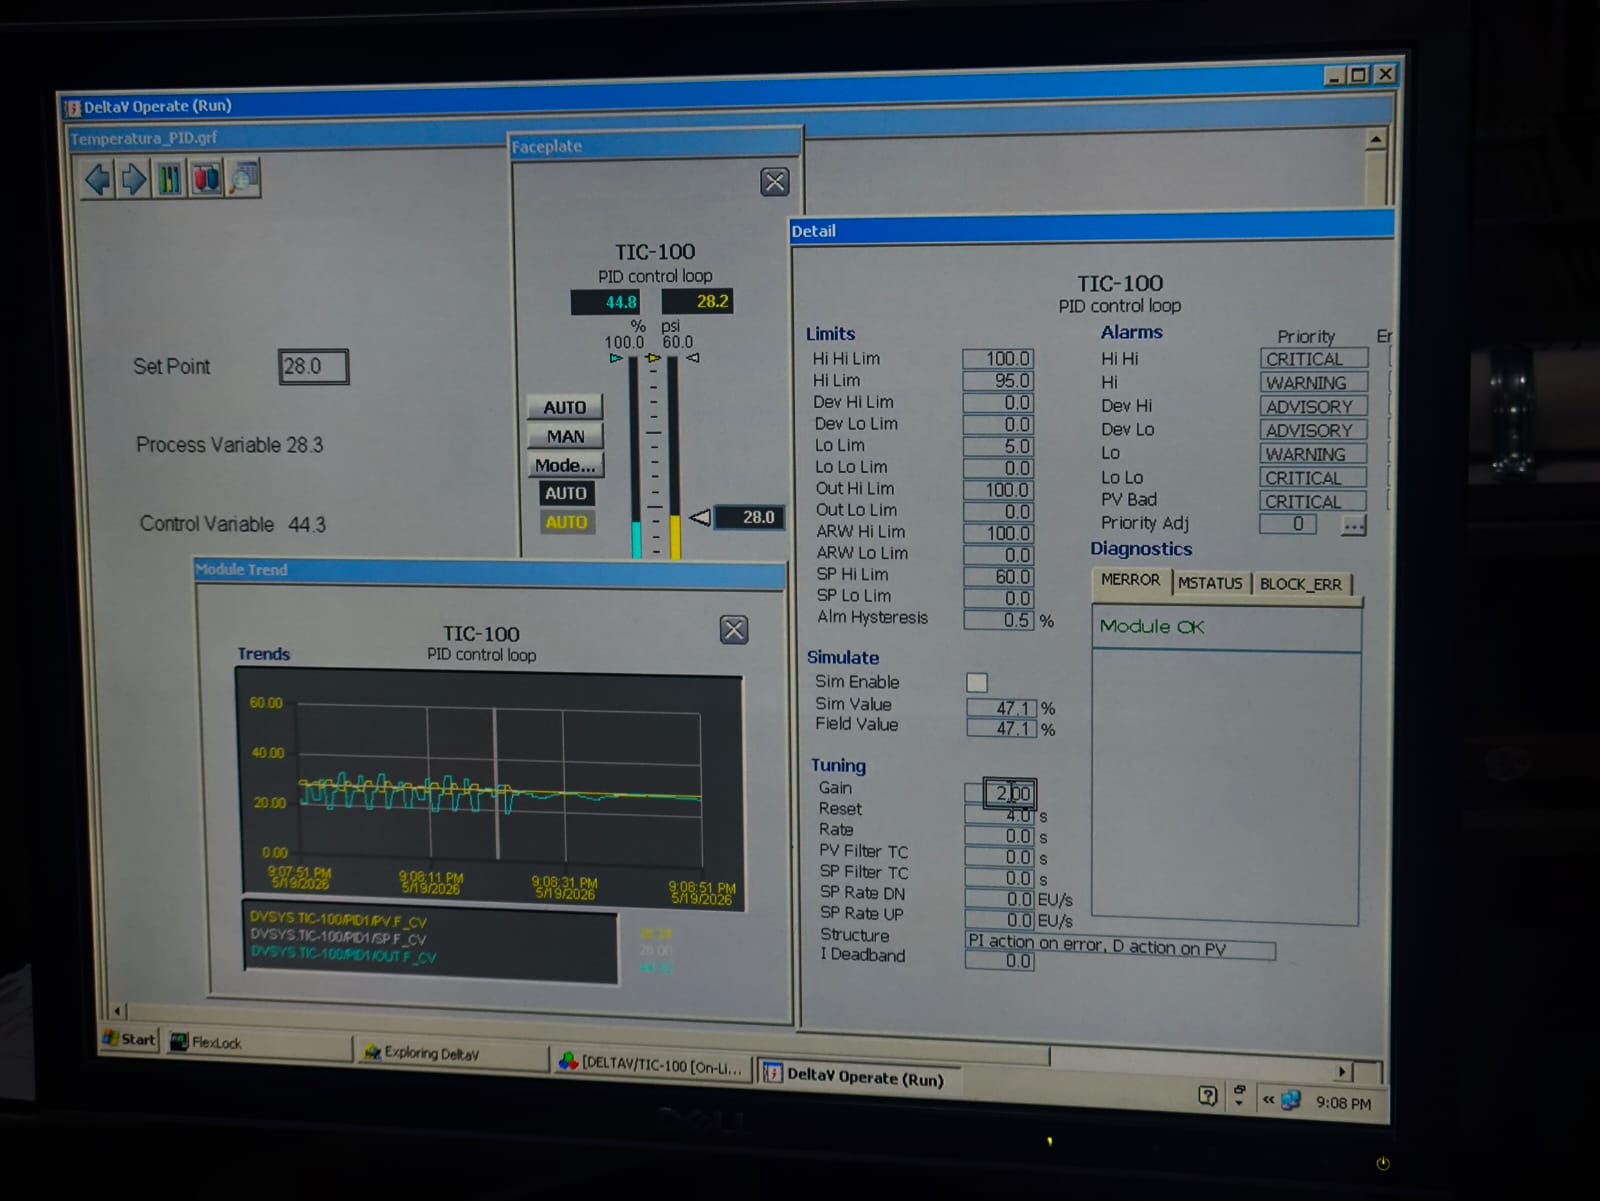
\includegraphics[width=0.92\textwidth]{figuras/hmi_tendencia_pid.jpeg}
\caption{Faceplate y tendencia del bloque PID en DeltaV durante la etapa de monitoreo}
\label{fig:hmi_tendencia}
\end{figure}

En la Figura \ref{fig:hmi_tendencia} se observa el \textit{faceplate} del controlador PID. La pantalla permite identificar el punto de ajuste, la variable de proceso, la salida de control y el modo de operación. También se observa la tendencia del lazo, útil para evaluar si la PV se acerca al SP, si existen oscilaciones y si la CV permanece dentro de un rango operativo razonable.

\begin{figure}[H]
\centering
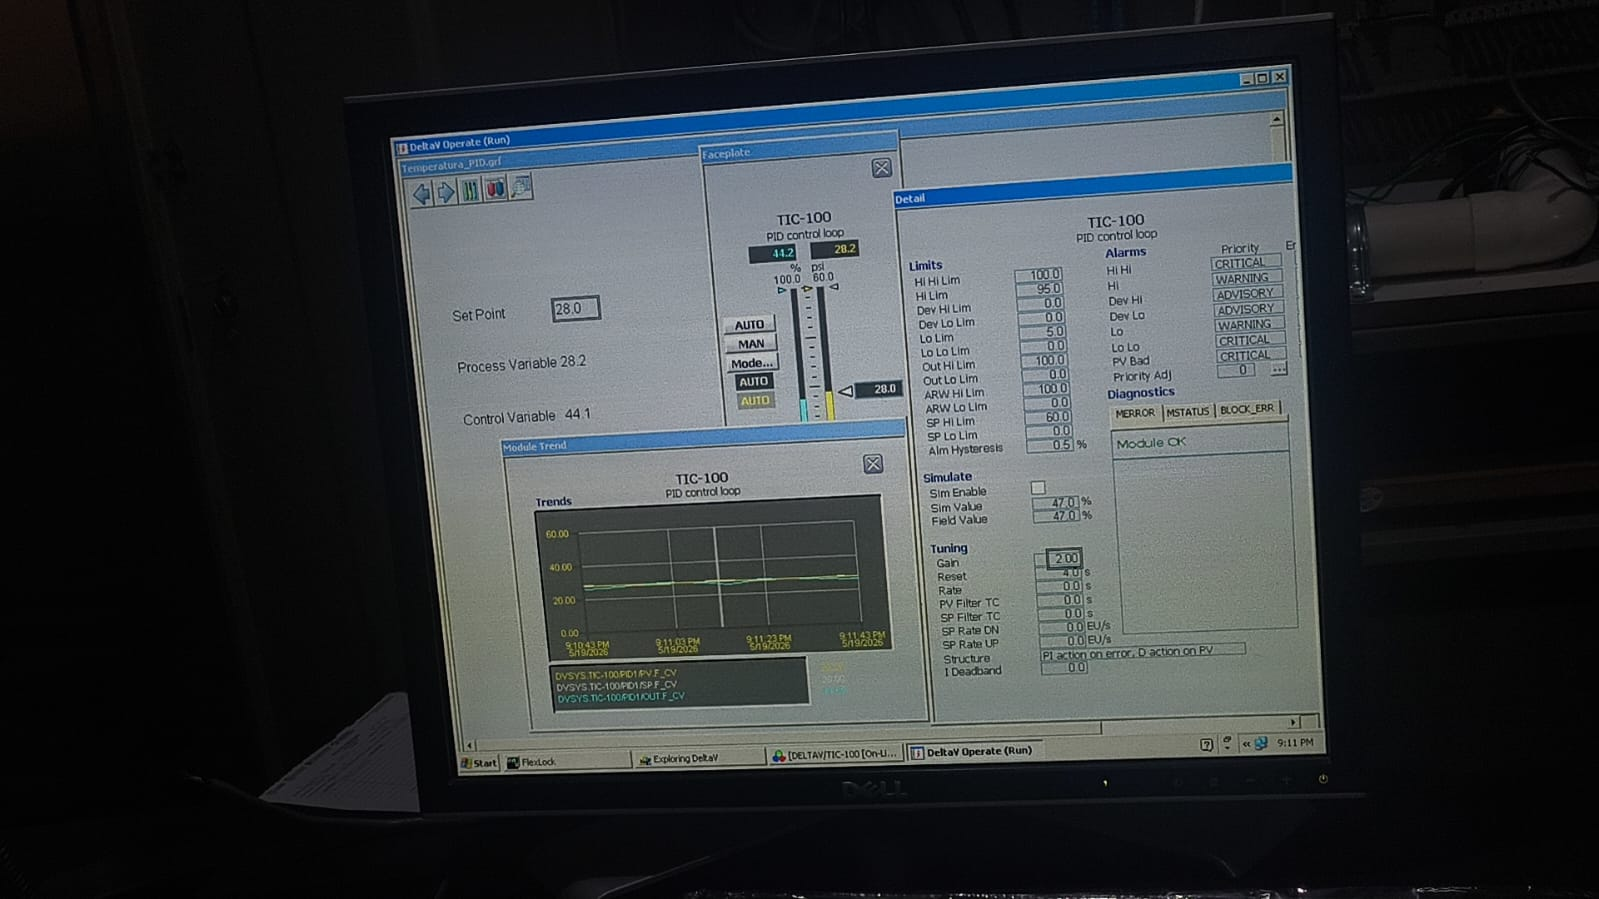
\includegraphics[width=0.92\textwidth]{figuras/hmi_operacion_estable.jpeg}
\caption{Condición de operación estable del lazo PID después de la sintonización}
\label{fig:hmi_estable}
\end{figure}

La Figura \ref{fig:hmi_estable} muestra una condición de operación estable después de la sintonización. La PV se mantiene cercana al set point y la salida del controlador se conserva en un valor intermedio, lo cual indica que la válvula no se encuentra saturada y todavía tiene capacidad para corregir perturbaciones en la entrada o salida de aire.

% -----------------------------------------------------------
\subsection*{Prueba de Límites del Sistema}

Finalmente se comprobaron los límites del sistema buscando un valor de set point que el banco fuera incapaz de alcanzar. Para ello se realizaron distintas pruebas, principalmente dentro del rango de 30 a 40 psia, donde el controlador podía funcionar adecuadamente. Al incrementar la exigencia del set point por encima de la capacidad disponible de entrada de aire, la variable de proceso dejaba de alcanzar el valor deseado y la salida del controlador tendía a elevarse, indicando que la válvula se aproximaba a su límite de acción.

Esta prueba permitió distinguir entre un problema de sintonía y una limitación física del proceso. Cuando la válvula, la presión de suministro o el flujo disponible no son suficientes, el controlador puede aumentar la salida, pero la PV no necesariamente alcanzará el SP. En ese caso, el error permanente no se corrige ajustando únicamente los parámetros PID, sino revisando la capacidad del sistema.

% -----------------------------------------------------------
\subsection*{Interpretación de la Respuesta del Controlador}

La respuesta observada indica que los parámetros de sintonía fueron adecuados para mantener una buena relación entre la variable de proceso, la variable de control y el set point. La etapa manual permitió encontrar una región de operación estable, mientras que el modo automático permitió comprobar que el PID podía corregir perturbaciones y sostener la presión deseada en el tanque pulmón.

\subsection*{Evidencia Fotográfica e Interpretación}

\begin{figure}[H]
\centering
\begin{minipage}{0.45\textwidth}
    \centering
    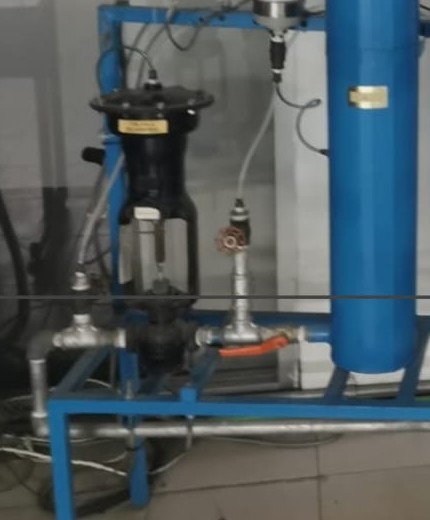
\includegraphics[height=7.0cm]{figuras/detalle_valvula.jpeg}
    \small (a) Válvula neumática de control
\end{minipage}
\hfill
\begin{minipage}{0.45\textwidth}
    \centering
    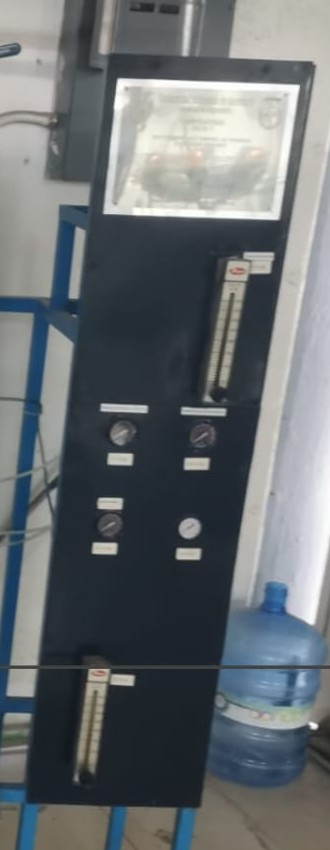
\includegraphics[height=7.0cm]{figuras/detalle_panel_rotametros.jpeg}
    \small (b) Panel de rotámetros y manómetros
\end{minipage}
\caption{Detalles de campo utilizados durante la sintonización del lazo}
\label{fig:detalles_campo}
\end{figure}

En la Figura \ref{fig:detalles_campo}(a) se observa la válvula neumática que actúa como elemento final de control. Su posición modifica el flujo de aire de entrada al tanque pulmón y, por lo tanto, permite que el controlador corrija la presión. En la Figura \ref{fig:detalles_campo}(b) se muestra el panel de rotámetros y manómetros; estos elementos permitieron establecer condiciones de entrada y salida, además de generar perturbaciones para probar la sintonía del PID.

\begin{figure}[H]
\centering
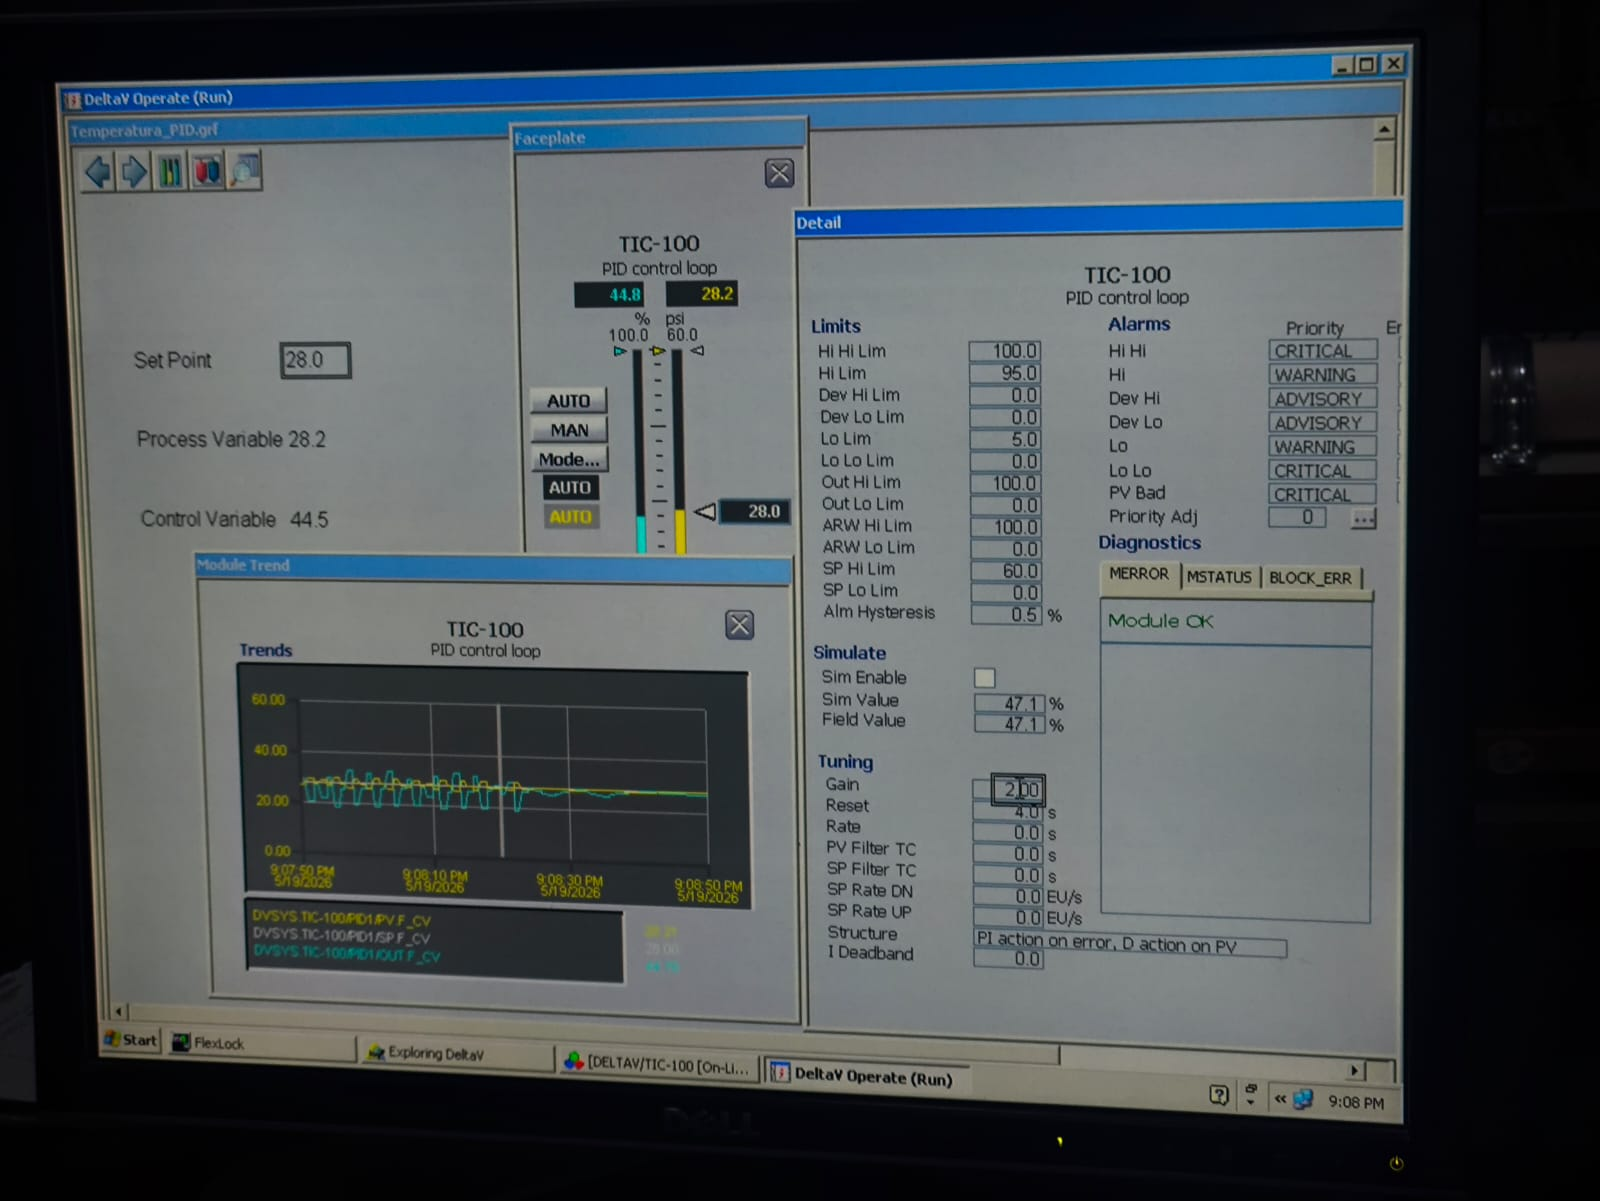
\includegraphics[width=0.92\textwidth]{figuras/hmi_prueba_pid.jpeg}
\caption{Monitoreo del lazo en DeltaV durante una prueba de operación}
\label{fig:hmi_prueba}
\end{figure}

En la Figura \ref{fig:hmi_prueba} se aprecia el seguimiento del lazo desde el DCS DeltaV. El \textit{faceplate} permite observar simultáneamente SP, PV y CV, además del modo de operación. Esta pantalla fue fundamental para decidir cuándo el sistema podía pasar de modo manual a modo automático y para detectar si la salida del controlador se acercaba a saturación durante las pruebas de límite.

\newpage

% ============================================================
% CUESTIONARIO
% ============================================================
\section*{Cuestionario}

\subsection*{1.- ¿En qué se basa o justifica la selección de los parámetros de cualquier sistema de control y cómo deberían ser los resultados obtenidos?}

La selección de parámetros de un sistema de control se justifica con base en la dinámica del proceso, el objetivo operativo, las restricciones de seguridad, el tipo de perturbaciones y la calidad de la medición. No existe una única combinación universal de $K_c$, $T_i$ y $T_d$; los parámetros deben seleccionarse de acuerdo con el comportamiento real del proceso.

En un lazo de presión como el del tanque pulmón, los parámetros se justifican por:

\begin{itemize}[itemsep=0.3em]
    \item La rapidez con la que cambia la presión ante variaciones de demanda.
    \item El volumen disponible del tanque y de la tubería.
    \item La capacidad de la válvula de suministro.
    \item El margen permitido antes de activar alarma o paro.
    \item La presencia de ruido en la medición del transmisor.
    \item El tiempo muerto del sistema neumático y del actuador.
\end{itemize}

Los resultados esperados deben mostrar estabilidad, presión cercana al punto de ajuste, recuperación ante perturbaciones, ausencia de oscilaciones sostenidas y una salida de controlador dentro de su rango normal de operación. En la práctica física, el sistema debía mantener la presión del tanque pulmón en el set point seleccionado, principalmente dentro del rango de 30--40 psia. Si el set point se colocaba fuera de la capacidad física del banco, la salida del controlador aumentaba, pero la variable de proceso no lograba alcanzar el valor deseado.

\subsection*{2.- Reporte escrito de toda la práctica}

El presente documento integra el marco conceptual de controladores, la selección del tipo de controlador, la configuración de parámetros PI, el dimensionamiento del tanque pulmón de nitrógeno, la práctica física realizada en el sistema de tanques de aire, la evidencia fotográfica del montaje, el DTI del sistema y el uso del DCS DeltaV durante la sintonización del lazo.

\subsection*{3.- Conclusiones}

El controlador es el elemento que permite transformar la medición de una variable de proceso en una acción correctiva sobre el elemento final de control. En sistemas de presión con tanque pulmón, el control PI es una opción adecuada porque combina respuesta proporcional con eliminación del error permanente, sin introducir la sensibilidad al ruido propia de la acción derivativa.

El análisis del caso teórico muestra que el margen de caída permitido, equivalente a solo 3\% de 115 psig, es muy pequeño para sostener un consumo de 40,000 SCFH durante 10 minutos únicamente con almacenamiento. El volumen calculado de aproximadamente 812.8 m$^3$ indica que el tanque pulmón no debe diseñarse como la única fuente de autonomía, sino como un elemento amortiguador complementado por un suministro continuo con capacidad suficiente.

La capacidad del suministro, de 80,000 SCFH, es el doble de la demanda nominal. Esto permite que el sistema pueda mantener la presión siempre que la válvula de control, el controlador y la estrategia de arranque estén correctamente configurados. La protección contra paro por baja presión debe lograrse mediante reserva de capacidad, arranque gradual, alarmas preventivas y ajuste adecuado del lazo.

En la práctica física se comprobó que el control de presión depende tanto de la sintonización del PID como de la capacidad real del proceso. El ajuste manual de los rotámetros permitió modificar la dinámica del sistema y encontrar una región donde la salida de control pudiera actuar sin saturarse. Después, al pasar el controlador a modo automático, el DCS DeltaV mantuvo la presión del tanque pulmón cercana al set point mediante la acción sobre el transductor I/P y la válvula de entrada de aire.

La prueba de límites mostró que, cuando se solicita un set point fuera de la capacidad del sistema, el controlador puede incrementar la salida pero no necesariamente lograr que la PV alcance el SP. Por ello, una buena respuesta de control requiere una relación adecuada entre PV, CV y SP, además de una instalación física con suficiente presión de suministro, rango de válvula y ajuste correcto de entrada y salida de aire.

\subsection*{Conclusiones Individuales}

\textbf{Luis Fernando Pérez Tellez.} La práctica permitió comprender que la sintonización de un controlador no depende únicamente de modificar valores en el PID, sino de conocer primero el comportamiento físico del proceso. Al ajustar los rotámetros y observar la respuesta del tanque pulmón, se identificó la importancia de trabajar dentro de una región donde la válvula conserve capacidad de acción.

\textbf{Jesus Pablo Arteaga Silva.} El uso del DCS DeltaV facilitó observar la relación entre el set point, la variable de proceso y la salida del controlador. El \textit{faceplate} del PID fue una herramienta clave para interpretar si el sistema respondía de manera estable y para decidir el momento adecuado de pasar de modo manual a modo automático.

\textbf{Braulio Iván Gómez Ortiz.} El sistema de tanques mostró que el volumen del proceso influye directamente en la dinámica de presión. El tanque pulmón ayudó a amortiguar cambios rápidos, mientras que la conexión con el tanque principal modificó la rapidez de respuesta. Esto confirma que la selección de parámetros debe considerar la capacidad y la inercia real del proceso.

\textbf{Joselyn Gallegos Abreo.} La prueba de límites permitió distinguir entre un problema de sintonización y una limitación física del sistema. Cuando el set point se colocó fuera de la capacidad del banco, el controlador incrementó su salida, pero la presión no pudo alcanzar el valor deseado. Esto demuestra que el control automático también depende del dimensionamiento correcto de los elementos de campo.

\textbf{Luis Alejandro Zeron Marin.} La práctica integró instrumentación, control e interpretación de diagramas de tubería e instrumentación. Replicar el DTI ayudó a relacionar cada componente físico con su función dentro del lazo: transmisor, controlador, transductor I/P, válvula y tanques. Con ello se reforzó la importancia de documentar el sistema antes de analizar su respuesta.

\newpage

\begin{thebibliography}{99}

\bibitem{smith2006}
Smith, C. A. y Corripio, A. B., \textit{Principles and Practice of Automatic Process Control}, 3rd edition, John Wiley \& Sons, Hoboken, NJ, USA, 2006.

\bibitem{ogata2010}
Ogata, K., \textit{Modern Control Engineering}, 5th edition, Prentice Hall, Upper Saddle River, NJ, USA, 2010.

\bibitem{creus2010}
Creus Solé, A., \textit{Instrumentación Industrial}, 8a edición, Marcombo, Barcelona, España, 2010.

\bibitem{liptak2006}
Lipták, B. G., \textit{Instrument Engineers' Handbook: Process Measurement and Analysis}, 4th edition, CRC Press, Boca Raton, FL, USA, 2003.

\bibitem{isa51}
ANSI/ISA-5.1-2009, \textit{Instrumentation Symbols and Identification}, International Society of Automation (ISA), Research Triangle Park, NC, USA, 2009.

\end{thebibliography}

\end{document}
